% Status: Erstkorrektur
% Produktdarstellung.tex
\subsection{Die Produktpräsentation}
Die Präsentation des Produktes basiert auf dem \emph{SVG}-Format welches von der React-Komponente \lstinline|SVGPageRenderer.tsx| im Ordner \lstinline|src/components/svgRenderers/| erzeugt wird. 
Durch Abbildung \ref{fig:Produktdarstellung} werden die Abhängigkeiten Produktdarstellung aufgezeigt. 
Zur Darstellung des Produktes gehören das Darstellen von Beschnittlinien, Falzlinien, Nutlinien, Bereichen die nicht bedruckbar sind, sowie Seitenbezeichnungen. 
Diese Elemente werden durch React-Komponenten im Ordner \lstinline|src/components/svgRenderers/pageAssets| dargestellt.
Bei einigen Produkten, Textilien oder Werbeprodukte, kann im Hintergrund eine Abbildung des Produktes dargestellt werden, welche durch die React-Komponente \lstinline|SVGProductImageRenderer.tsx| erzeugt wird. 

Für die Produktdarstellung wird der Komponente eine Produktbeschreibung übergeben, deren Struktur durch die Datei \lstinline|src/core/entities/product/Product.ts| definiert ist.

Innerhalb des FreeDesign-Editors kann die Darstellung der Produktseite, rotiert, skaliert und verschoben werden. Für diese Aufgaben ist die React-Komponente \lstinline|PagePresenter.tsx| verantwortlich. 
Zur Berechnung der Darstellungsmöglichkeiten nutzt die Komponente mathematische Funktionen aus der Datei \lstinline|FDMath.ts| welche im Ordner \lstinline|src/core/helpers| enthalten ist. 
Zwischen der Datei \lstinline|FDMath.ts| und \lstinline|point.ts| besteht eine zyklische Abhängigkeit. Dies durch die beiden roten Pfeile, mit je einem Kreis, dargestellt.

% Wie von Abbildung \ref{fig:Produktdarstellung} zu entnehmen ist, werden für das Erzeugen der \emph{SVG}-Struktur \emph{ReactJS}-Komponenten genutzt, die exklusiv für die Produktdarstellung erstellt wurden. Diese Komponenten finden in keinem anderem Zusammenhang Verwendung und sind eng an die Produktdarstellung gekoppelt. 
% 

% Das Produkt wird durch eine Struktur beschrieben, welche im \emph{core}-Ordner hinterlegt ist. Die Struktur enthält sowohl geometrische Information für die Produktdarstellung, als auch Produktspezifische eigenschaften, wie die Existenz von Beschnittlinien. 

% Für die Darstellung innerhalb des FreeDesign-Editors ist die Nutzung von mathematischen Operationen notwendig, die im Anwendungskern definiert sind. 

% Der Produktdarstellung kann ein Kindelement übergeben werden, welches in die die Produktdarstellung eingebettet werden. 

\begin{figure}[H]
    \centering
    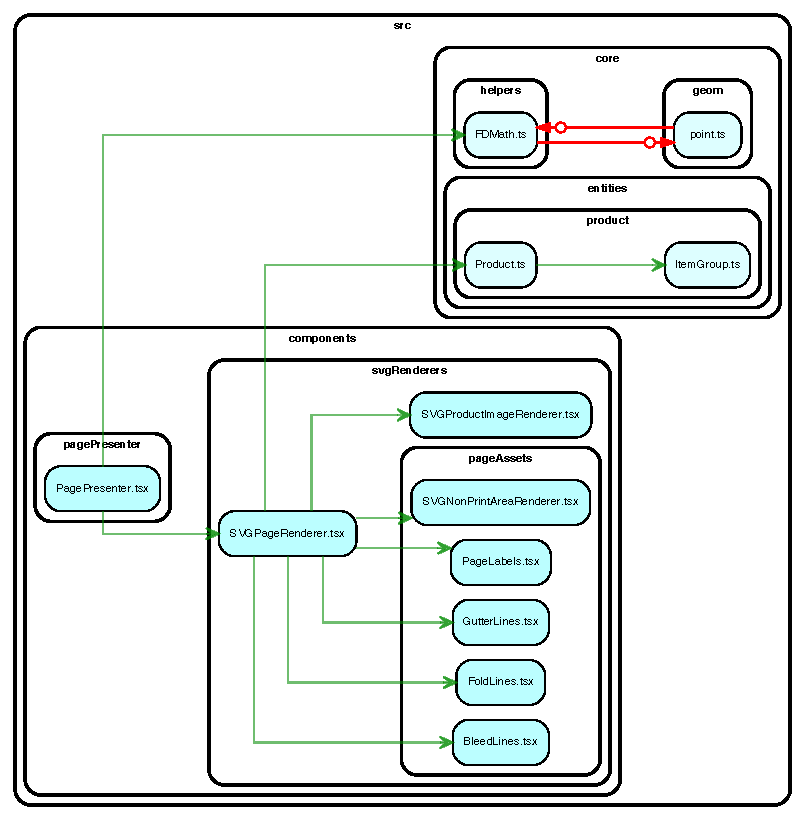
\includegraphics{diagrams/Ist-Architektur/page-presenter-analysis.pdf}
    \caption{Abhängigkeiten der Komponenten für Produktdarstellung}
    \label{fig:Produktdarstellung}
\end{figure}

Für die Produktdarstellung wurden die folgende drei Bausteine identifiziert.
\begin{multicols}{3}
    \begin{enumerate}
\item{Mathematik}
\item{Produktdarstellung}
\item{Produktstruktur} 
\end{enumerate} 
\end{multicols}